\documentclass[12pt, a4paper, oneside]{article}
\usepackage{graphicx}
\usepackage{arial}
\renewcommand{\familydefault}{\sfdefault}
\usepackage[T1]{fontenc}
\usepackage[polish]{babel}
\usepackage[utf8]{inputenc}
\usepackage{lmodern}
\usepackage[left=2cm,right=2cm,top=2cm,bottom=2cm]{geometry}
\selectlanguage{polish}
\usepackage{booktabs, multicol, multirow}
\usepackage{longtable}

\begin{document}
\section{Wykorzystane wzory}
Niepewność zmierzonego prądu (Metex M-3800, AC, zakres 20 A)
\begin{equation}
u(I)=2\%~ rdg + 5~ dgt
\end{equation}
Niepewność zmierzonego napięcia (Metex M-3850, DC, zakres 40 V)
\begin{equation}
u(U)=0.3\%~ rdg + 1~ dgt
\end{equation}
Okres drgań wahadła
\begin{equation}
T=\frac{t_n}{n}
\end{equation}
Niepewność wyznaczonego okresu drgań wahadła
\begin{equation}
u(T)=\frac{\sqrt{\frac{\Delta^2_{obserwatora}}{3} + \frac{\Delta^2_{stopera}}{3}}}{n}
\end{equation}
Częstość własna drgań wahadła
\begin{equation}
\omega = \frac{2\cdot \pi}{T}
\end{equation}
Niepewność częstości własnej drgań wahadła
\begin{equation}
u_C(\omega)=\sqrt{(\frac{\partial \omega}{\partial T})^2 \cdot u^2(T)} = \frac{2\cdot\pi}{T}\cdot u(T)
\end{equation}
Logarytmiczny dekrement tłumienia
\begin{equation}
\Lambda=ln(\frac{A_n}{A_{n+1}})
\end{equation}
Niepewność wyznaczonego logarytmicznego dekrementu tłumienia
\begin{equation}
u_C(\Lambda)=\sqrt{(\frac{\partial \Lambda}{\partial A_n})^2\cdot u^2(A_n) + (\frac{\partial \Lambda}{\partial A_{n+1}})^2\cdot u^2(A_{n+1})}=\sqrt{\frac{u^2(A_n)}{A_n^2}+\frac{u^2(A_{n+1})}{A_{n+1}^2}}
\end{equation}
Dobroć układu
\begin{equation}
Q=\frac{\omega_r}{\Delta\omega}
\end{equation}
Niepewność wyznaczonej dobroci układu
\begin{equation}
u_C(Q)=\sqrt{\frac{\partial Q}{\partial\omega_r}\cdot u^2(\omega_r) + \frac{\partial Q}{\partial\Delta\omega}\cdot u^2(\Delta\omega)}=\sqrt{\frac{u^2(\omega_r)}{(\Delta\omega)^2}+\frac{\omega^2_r}{(\Delta\omega)^4}\cdot u^2(\Delta\omega)}
\end{equation}
\clearpage
\section{Przykładowe obliczenia}
Niepewność zmierzonego prądu (Metex M-3800, AC, zakres 20 A)
\begin{center}
$u(I)=2\% \cdot 0.46 + 5\cdot0.01=0.06$
\end{center}
Niepewność zmierzonego napięcia (Metex M-3850, DC, zakres 40 V)
\begin{center}
$u(U)=0.3\% \cdot 1.985 + 1\cdot 0.001=0.007$
\end{center}
Okres drgań wahadła
\begin{center}
$T=\frac{19.31}{10}=1.931~[s]$
\end{center}
Niepewność wyznaczonego okresu drgań wahadła
\begin{center}
$u(T)=\frac{\sqrt{\frac{(0.2)^2}{3} + \frac{(0.01)^2}{3}}}{10}=0.012~[s]$
\end{center}
Częstość własna drgań wahadła
\begin{center}
$\omega=\frac{2\cdot\pi}{1.931}=3.25~[\frac{rad}{s}]$
\end{center}
Niepewność wyznaczonej częstości własnej drgań wahadła
\begin{center}
$u_C(\omega) = \frac{2\cdot\pi}{1.931}\cdot0.012=0.04~[\frac{rad}{s}]$
\end{center}
Logarytmiczny dekrement tłumienia
\begin{center}
$\Lambda=ln(\frac{7.8}{7})=0.108$
\end{center}
Niepewność wyznaczonego logarytmicznego dekrementu tłumienia
\begin{center}
$u_C(\Lambda)=\sqrt{\frac{(0.058)^2}{7.8} + \frac{(0.058)^2}{7}}=0.012$
\end{center}
Dobroć układu
\begin{center}
$Q = \frac{3.3}{0.46}=7.17$
\end{center}
Niepewność wyznaczonej dobroci układu
\begin{center}
$u_C(Q) = \sqrt{\frac{(0.1)^2}{(0.46)^2} + \frac{(3.3)^2}{(0.46)^4}\cdot(0.025)^2}=0.45$
\end{center}
\section{Wyniki pomiarów i opracowanie}
% Table generated by Excel2LaTeX from sheet 'Arkusz1'
\begin{table}[h]
  \centering
  \caption{Okres drgań oraz częstość własna drgań wahadła przy wychyleniu początkowym $\alpha_0$}
    \begin{tabular}{|c|c|c|c|c|c|}\hline
    \multicolumn{1}{|c|}{$\alpha_0~[dz]$} & \multicolumn{1}{c|}{$t_{10}~[s]$} & \multicolumn{1}{c|}{$T~[s]$} & \multicolumn{1}{c|}{$u(T)~[s]$} & \multicolumn{1}{c|}{$\omega~[\frac{rad}{s}]$} & \multicolumn{1}{c|}{$u_C(\omega)~[\frac{rad}{s}]$} \\\hline
    2 & 19.31 & 1.931 & 0.012 & 3.25 & 0.04 \\\hline
    6 & 19.41 & 1.941 & 0.012 & 3.237 & 0.039 \\\hline
    10 & 19.34 & 1.934 & 0.012 & 3.249 & 0.039 \\\hline
    \end{tabular}%
\end{table}%
\clearpage
\begin{figure}[h]
\centering
\caption{Wykres funkcji A = f(t) dla pomiarów bez prądu hamującego}
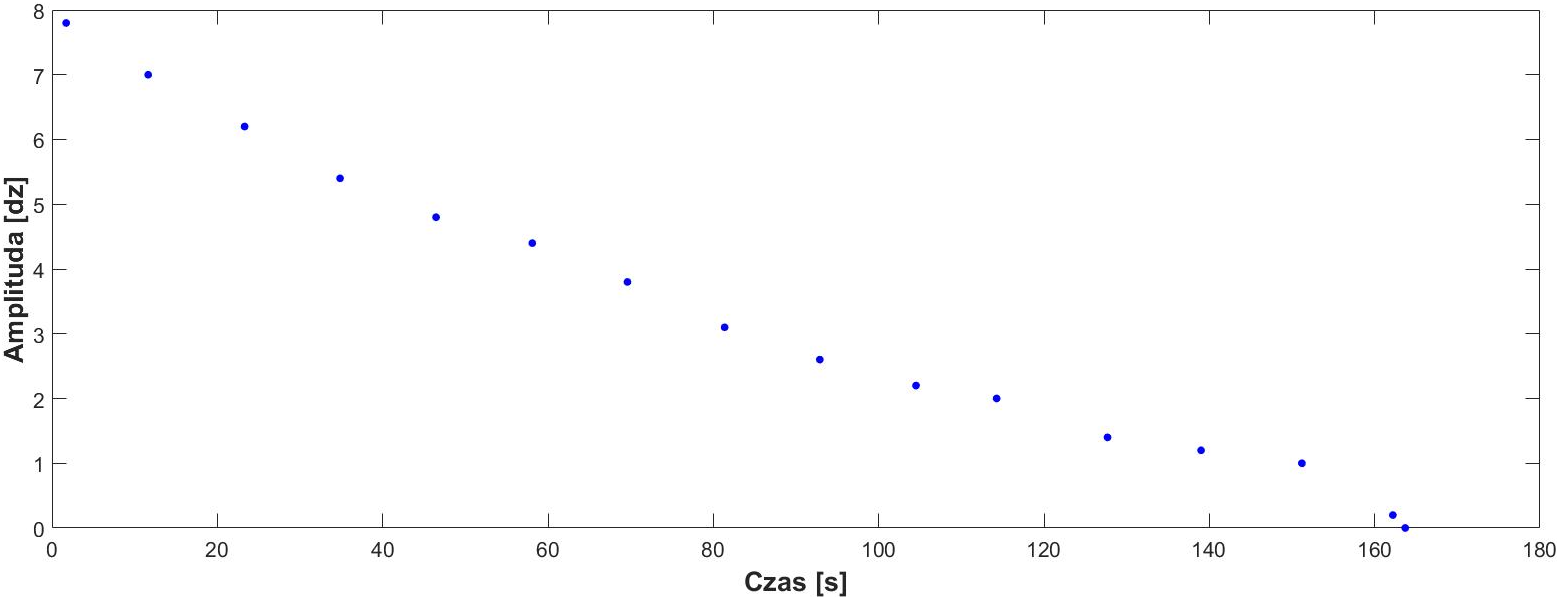
\includegraphics[scale=0.3]{f1.png}
\end{figure}
% Table generated by Excel2LaTeX from sheet 'Arkusz1'
\begin{table}[h]
  \centering
  \caption{Ilość okresów, amplituda, czas oraz logarytmiczny dekrement tłumienia przy $\alpha_0$ = 8 [dz], dla pomiarów bez prądu hamującego}
    \begin{tabular}{|c|c|c|c|c|c|c|}\hline
    $n$ & $A~[dz]$ & $u(A)~[dz]$ & $t~[s]$ & \multicolumn{1}{c|}{$u(t)~[s]$} & $\Lambda$ & \multicolumn{1}{c|}{$u_C(\Lambda)$} \\\hline
    1 & 7.800 & 0.058 & 1.71 & 0.12 & 0.108 & \multicolumn{1}{c|}{0.012} \\\hline
    6 & 7.000 & 0.058 & 11.63 & 0.12 & 0.121 & \multicolumn{1}{c|}{0.013} \\\hline
    12 & 6.200 & 0.058 & 23.30 & 0.12 & 0.138 & \multicolumn{1}{c|}{0.015} \\\hline
    18 & 5.400 & 0.058 & 34.84 & 0.12 & 0.118 & \multicolumn{1}{c|}{0.017} \\\hline
    24 & 4.800 & 0.058 & 46.46 & 0.12 & 0.087 & \multicolumn{1}{c|}{0.018} \\\hline
    30 & 4.400 & 0.058 & 58.10 & 0.12 & 0.147 & \multicolumn{1}{c|}{0.021} \\\hline
    36 & 3.800 & 0.058 & 69.61 & 0.12 & 0.204 & \multicolumn{1}{c|}{0.025} \\\hline
    42 & 3.100 & 0.058 & 81.37 & 0.12 & 0.176 & \multicolumn{1}{c|}{0.029} \\\hline
    48 & 2.600 & 0.058 & 92.88 & 0.12 & 0.167 & \multicolumn{1}{c|}{0.035} \\\hline
    54 & 2.200 & 0.058 & 104.52 & 0.12 & 0.10 & \multicolumn{1}{c|}{0.04} \\\hline
    60 & 2.000 & 0.058 & 114.27 & 0.12 & 0.357 & \multicolumn{1}{c|}{0.051} \\\hline
    66 & 1.400 & 0.058 & 127.68 & 0.12 & 0.154 & \multicolumn{1}{c|}{0.064} \\\hline
    72 & 1.200 & 0.058 & 139.00 & 0.12 & 0.182 & \multicolumn{1}{c|}{0.076} \\\hline
    78 & 1.000 & 0.058 & 151.20 & 0.12 & - & - \\\hline
    84 & 0.200 & 0.058 & 162.20 & 0.12 & - & - \\\hline
    85 & 0.000 & 0.058 & 163.70 & 0.12 & - & - \\\hline
    \end{tabular}%
  \label{tab:addlabel}%
\end{table}%
\noindent{\bf Uśredniona wartość logarytmicznego dekrementu tłumienia:}
\begin{center}
$\bar{\Lambda}$ = 0.158 $\pm$ 0.011
\end{center}
\clearpage
\begin{figure}[h]
\centering
\caption{Wykres funkcji A = f(t) dla pomiarów przy prądzie hamującym I$_1$ = (0.46 $\pm$ 0.06) A}
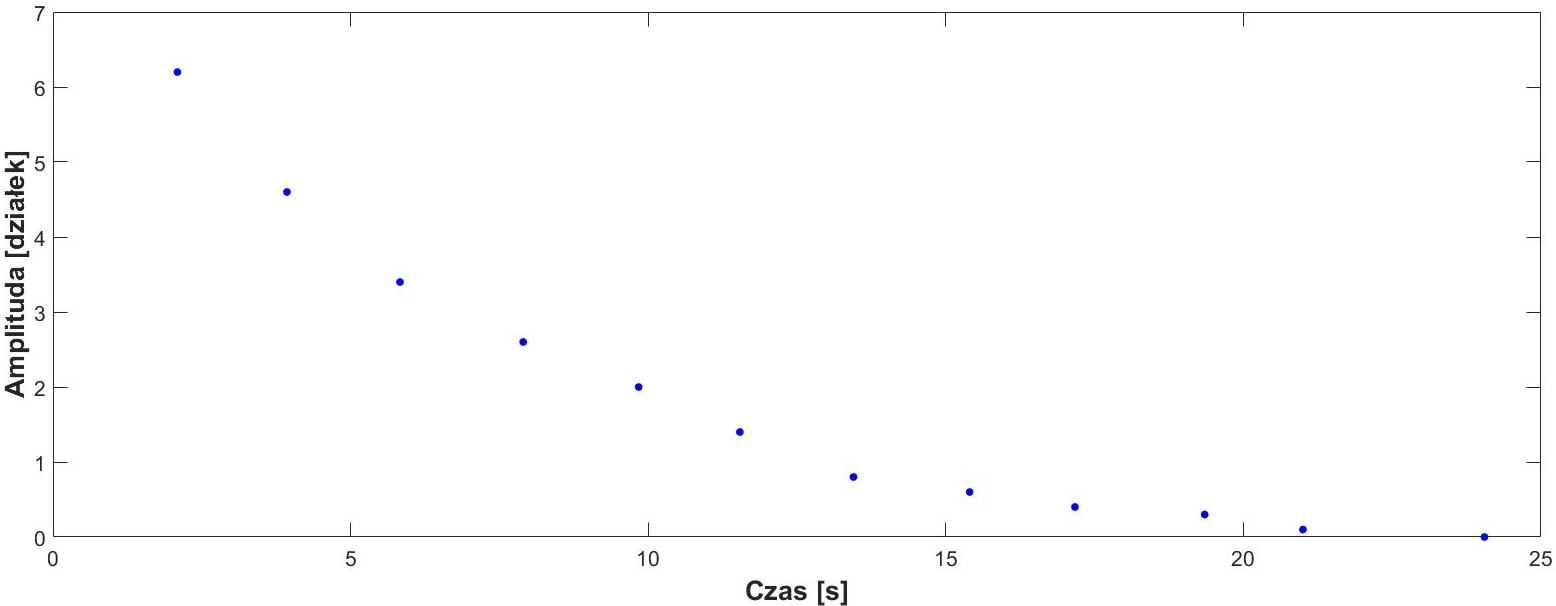
\includegraphics[scale=0.3]{f2.png}
\end{figure}
% Table generated by Excel2LaTeX from sheet 'Arkusz1'
\begin{table}[h]
  \centering
  \caption{Ilość okresów, amplituda, czas oraz logarytmiczny dekrement tłumienia przy $\alpha_0$ = 8 [dz] i prądzie hamującym I$_1$ = (0.46 $\pm$ 0.06) A}
    \begin{tabular}{|c|c|c|c|c|c|c|}\hline
    $n$ & $A~[dz]$ & $u(A)~[dz]$ & $t~[s]$ & \multicolumn{1}{|c|}{$u(t)~[s]$} & $\Lambda$ & $u_C(\Lambda)$ \\\hline
    1 & 6.200 & 0.058 & 2.09 & 0.12 & 0.298 & 0.016 \\\hline
    2 & 4.600 & 0.058 & 3.93 & 0.12 & 0.302 & 0.022 \\\hline
    3 & 3.400 & 0.058 & 5.83 & 0.12 & 0.268 & 0.028 \\\hline
    4 & 2.600 & 0.058 & 7.90 & 0.12 & 0.262 & 0.037 \\\hline
    5 & 2.000 & 0.058 & 9.84 & 0.12 & 0.357 & 0.051 \\\hline
    6 & 1.400 & 0.058 & 11.54 & 0.12 & 0.560 & 0.084 \\\hline
    7 & 0.800 & 0.058 & 13.45 & 0.12 & 0.29 & 0.13 \\\hline
    8 & 0.600 & 0.058 & 15.40 & 0.12 & 0.41 & 0.18 \\\hline
    9 & 0.400 & 0.058 & 17.17 & 0.12 & 0.29 & 0.25 \\\hline
    10 & 0.300 & 0.058 & 19.35 & 0.12 & - & - \\\hline
    11 & 0.100 & 0.058 & 21.00 & 0.12 & - & - \\\hline
    12 & 0.000 & 0.058 & 24.05 & 0.12 & - & - \\\hline
    \end{tabular}%
  \label{tab:addlabel}%
\end{table}%
\noindent{\bf Uśredniona wartość logarytmicznego dekrementu tłumienia:}
\begin{center}
$\bar{\Lambda}$ = 0.34 $\pm$ 0.04
\end{center}
\clearpage
\begin{figure}[h]
\centering
\caption{Wykres funkcji A = f(t) dla pomiarów przy prądzie hamującym I$_2$ = (0.400 $\pm$ 0.058) A}
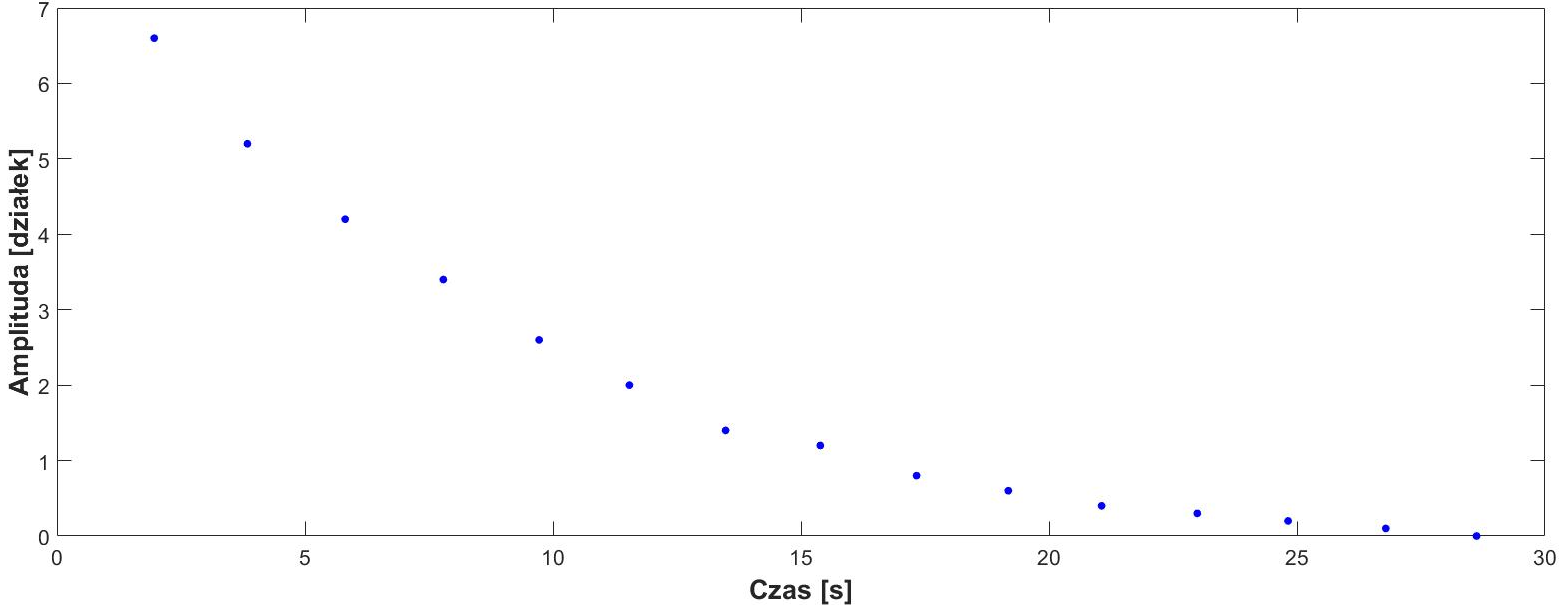
\includegraphics[scale=0.3]{f3.png}
\end{figure}
% Table generated by Excel2LaTeX from sheet 'Arkusz1'
\begin{table}[h]
  \centering
  \caption{Ilość okresów, amplituda, czas oraz logarytmiczny dekrement tłumienia przy $\alpha_0$ = 8 [dz] i prądzie hamującym I$_2$ = (0.400 $\pm$ 0.058) A}
    \begin{tabular}{|c|c|c|c|c|c|c|}\hline
    $n$ & $A~[dz]$ & $u(A)~[dz]$ & $t~[s]$ & $u(t)~[s]$ & $\Lambda$ & $u_C(\Lambda)$ \\\hline
    1 & 6.600 & 0.058 & 1.96 & 0.12 & 0.238 & 0.015 \\\hline
    2 & 5.200 & 0.058 & 3.84 & 0.12 & 0.214 & 0.018 \\\hline
    3 & 4.200 & 0.058 & 5.81 & 0.12 & 0.211 & 0.022 \\\hline
    4 & 3.400 & 0.058 & 7.79 & 0.12 & 0.268 & 0.029 \\\hline
    5 & 2.600 & 0.058 & 9.72 & 0.12 & 0.262 & 0.037 \\\hline
    6 & 2.000 & 0.058 & 11.54 & 0.12 & 0.357 & 0.051 \\\hline
    7 & 1.400 & 0.058 & 13.48 & 0.12 & 0.154 & 0.064 \\\hline
    8 & 1.200 & 0.058 & 15.39 & 0.12 & 0.405 & 0.088 \\\hline
    9 & 0.800 & 0.058 & 17.33 & 0.12 & 0.29 & 0.13 \\\hline
    10 & 0.600 & 0.058 & 19.18 & 0.12 & 0.41 & 0.18 \\\hline
    11 & 0.400 & 0.058 & 21.06 & 0.12 & 0.29 & 0.25 \\\hline
    12 & 0.300 & 0.058 & 22.99 & 0.12 & 0.41 & 0.35 \\\hline
    13 & 0.200 & 0.058 & 24.82 & 0.12 & - & - \\\hline
    14 & 0.100 & 0.058 & 26.79 & 0.12 & - & - \\\hline
    15 & 0.000 & 0.058 & 28.62 & 0.12 & - & - \\\hline
    \end{tabular}%
  \label{tab:addlabel}%
\end{table}%
\noindent{\bf Uśredniona wartość logarytmicznego dekrementu tłumienia:}
\begin{center}
$\bar{\Lambda}$ = 0.29 $\pm$ 0.15
\end{center}
\begin{figure}[h]
\centering
\caption{Wykres funkcji $\omega$ = f(U) i przybliżenie najlepszą prostą dla pomiarów przy prądzie hamującym I = (0.400 $\pm$ 0.058) A}
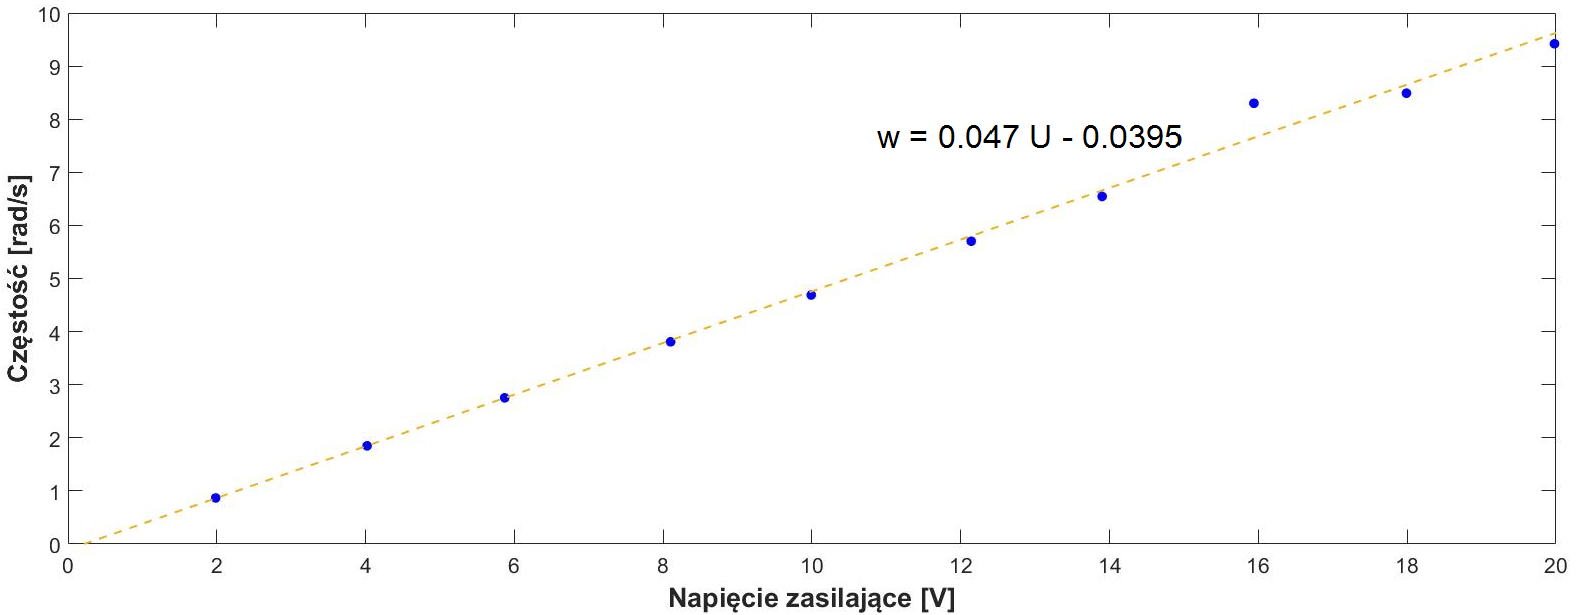
\includegraphics[scale=0.3]{f4.png}
\end{figure}
% Table generated by Excel2LaTeX from sheet 'Arkusz1'
\begin{table}[h]
  \centering
  \caption{Ilość obrotów silniczka, napięcie zasilające, czas obrotów, okres, częstość silniczka przy prądzie hamującym I = (0.400 $\pm$ 0.058) A}
    \begin{tabular}{|c|c|c|c|c|c|c|c|c|}\hline
    $n$ & $U~[V]$ & $u(U)~[V]$ & $t~[s]$ & $u(t)~[s]$ & $T~[s]$ & $u(T)~[s]$ & $\omega~[\frac{rad}{s}]$ & $u_C(\omega)~[\frac{rad}{s}]$
 \\\hline
    5 & 1.985 & 0.007 & 36.23 & 0.12 & 7.246 & 0.024 & 0.867 & 0.021 \\\hline
    5 & 4.020 & 0.014 & 16.99 & 0.12 & 3.398 & 0.024 & 1.849 & 0.045 \\\hline
    5 & 5.870 & 0.019 & 11.41 & 0.12 & 2.282 & 0.024 & 2.753 & 0.067 \\\hline
    5 & 8.100 & 0.026 & 8.25 & 0.12 & 1.650 & 0.024 & 3.808 & 0.092 \\\hline
    10 & 9.990 & 0.031 & 13.40 & 0.12 & 1.340 & 0.012 & 4.689 & 0.057 \\\hline
    10 & 12.140 & 0.038 & 11.02 & 0.12 & 1.102 & 0.012 & 5.702 & 0.069 \\\hline
    10 & 13.900 & 0.043 & 9.60 & 0.12 & 0.960 & 0.012 & 6.545 & 0.079 \\\hline
    10 & 15.940 & 0.049 & 7.57 & 0.12 & 0.757 & 0.012 & 8.3 & 0.1 \\\hline
    10 & 17.990 & 0.055 & 7.40 & 0.12 & 0.740 & 0.012 & 8.49 & 0.11 \\\hline
    10 & 19.980 & 0.061 & 6.67 & 0.12 & 0.667 & 0.012 & 9.42 & 0.12 \\\hline
    \end{tabular}%
  \label{tab:addlabel}%
\end{table}%
\begin{figure}[h]
\centering
\clearpage
\caption{Wykres funkcji $\omega$ = f(U) i przybliżenie najlepszą prostą dla pomiarów przy prądzie hamującym I = (0.450 $\pm$ 0.059) A}
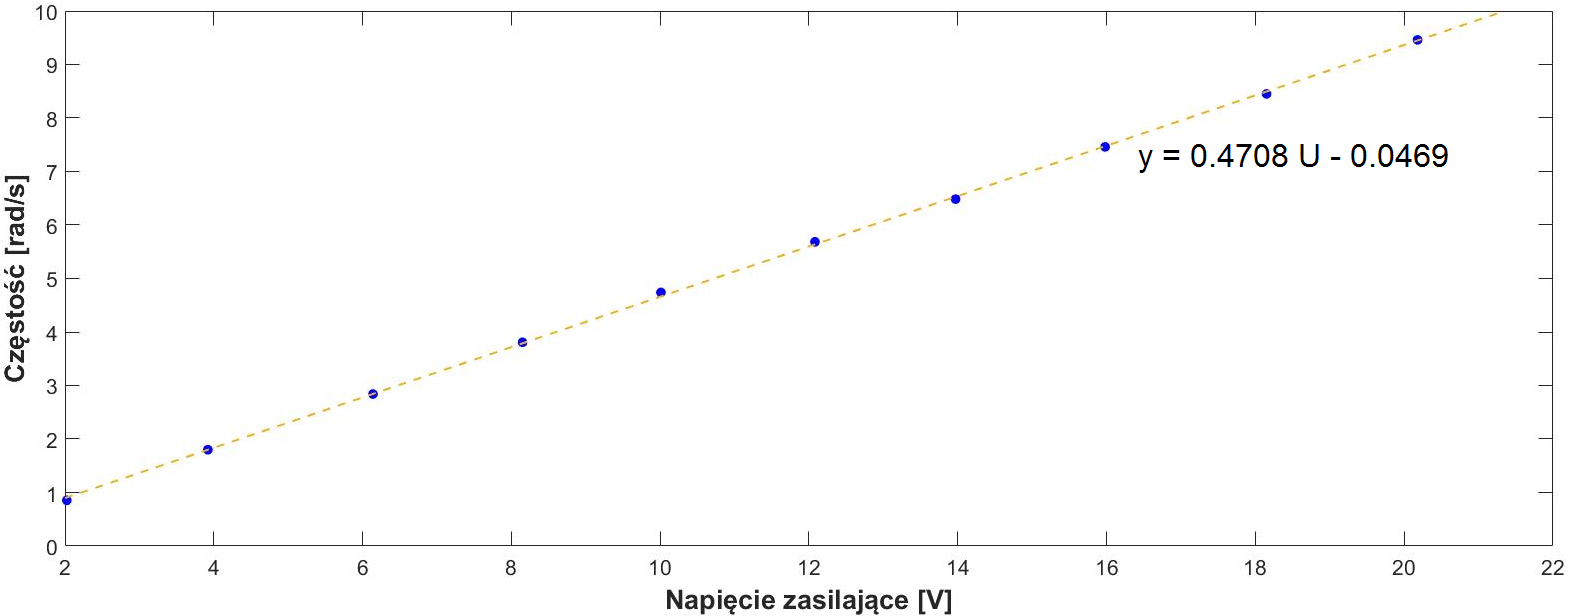
\includegraphics[scale=0.3]{f5.png}
\end{figure}
% Table generated by Excel2LaTeX from sheet 'Arkusz1'
\begin{table}[h]
  \centering
  \caption{Ilość obrotów silniczka, napięcie zasilające, czas obrotów, okres, częstość silniczka przy prądzie hamującym I = (0.450 $\pm$ 0.059) A}
    \begin{tabular}{|c|c|c|c|c|c|c|c|c|}\hline
    $n$ & $U~[V]$ & $u(U)~[V]$ & $t~[s]$ & $u(t)~[s]$ & $T~[s]$ & $u(T)~[s]$ & $\omega~[\frac{rad}{s}]$ & $u_C(\omega)~[\frac{rad}{s}]$ \\\hline
    5 & 2.025 & 0.007 & 36.80 & 0.12 & 7.360 & 0.024 & 0.854 & 0.021 \\\hline
    5 & 3.920 & 0.013 & 17.46 & 0.12 & 3.492 & 0.024 & 1.799 & 0.044 \\\hline
    5 & 6.140 & 0.020 & 11.06 & 0.12 & 2.212 & 0.024 & 2.840 & 0.069 \\\hline
    5 & 8.150 & 0.026 & 8.25 & 0.12 & 1.650 & 0.024 & 3.808 & 0.092 \\\hline
    5 & 10.010 & 0.031 & 6.63 & 0.12 & 1.326 & 0.024 & 4.74 & 0.12 \\\hline
    10 & 12.080 & 0.037 & 11.05 & 0.12 & 1.105 & 0.012 & 5.686 & 0.069 \\\hline
    10 & 13.970 & 0.043 & 9.69 & 0.12 & 0.969 & 0.012 & 6.484 & 0.078 \\\hline
    10 & 15.980 & 0.049 & 8.42 & 0.12 & 0.842 & 0.012 & 7.46 & 0.09 \\\hline
    10 & 18.150 & 0.056 & 7.44 & 0.12 & 0.744 & 0.012 & 8.45 & 0.11 \\\hline
    10 & 20.180 & 0.062 & 6.64 & 0.12 & 0.664 & 0.012 & 9.46 & 0.12 \\\hline
    \end{tabular}%
  \label{tab:addlabel}%
\end{table}%
\begin{figure}[h]
\centering
\caption{Wykres funkcji $\omega$ = f(U) i przybliżenie najlepszą prostą dla pomiarów przy prądzie hamującym I = (0.50 $\pm$ 0.06) A}
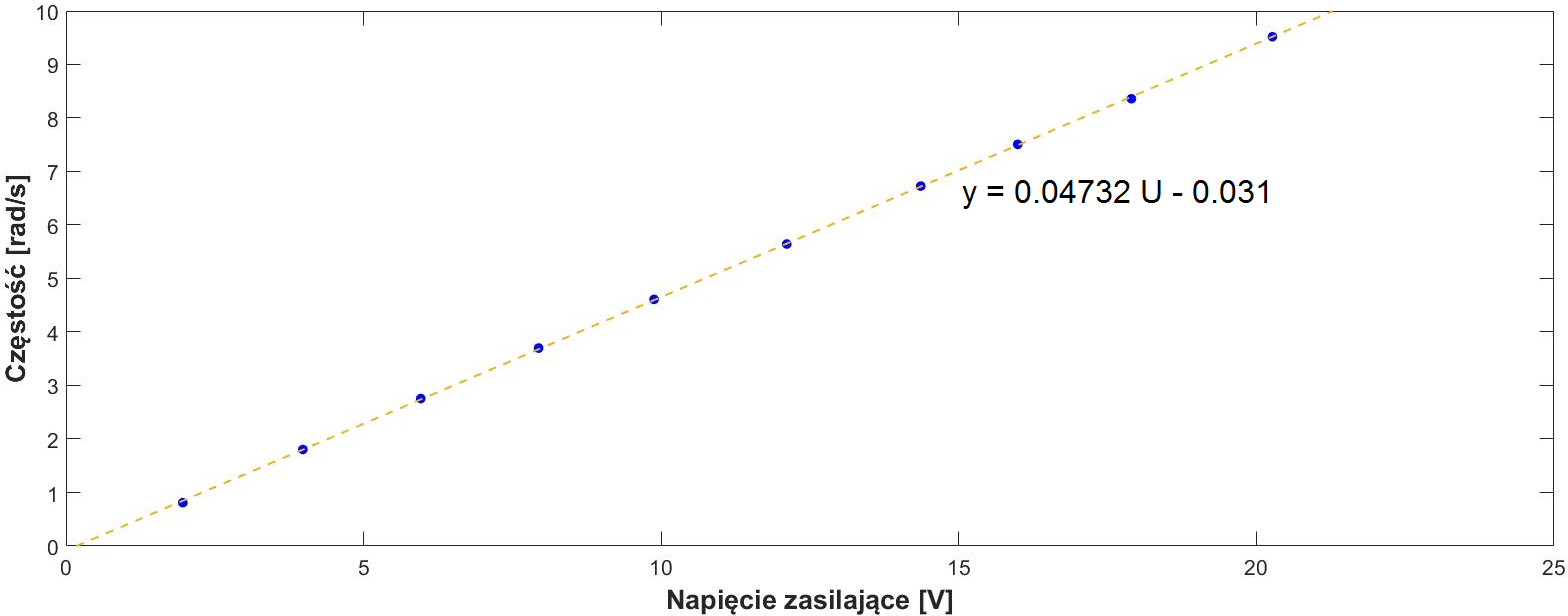
\includegraphics[scale=0.3]{f6.png}
\end{figure}
% Table generated by Excel2LaTeX from sheet 'Arkusz1'
\begin{table}[h]
  \centering
  \caption{Ilość obrotów silniczka, napięcie zasilające, czas obrotów, okres, częstość silniczka przy prądzie hamującym I = (0.50 $\pm$ 0.06) A}
    \begin{tabular}{|c|c|c|c|c|c|c|c|c|}\hline
    $n$ & $U~[V]$ & $u(U)~[V]$ & $t~[s]$ & $u(t)~[s]$ & $T~[s]$ & $u(T)~[s]$ & $\omega~[\frac{rad}{s}]$ & $u_C(\omega)~[\frac{rad}{s}]$ \\\hline
    5 & 1.963 & 0.007 & 38.60 & 0.12 & 7.720 & 0.024 & 0.81 & 0.02 \\\hline
    5 & 3.980 & 0.013 & 17.41 & 0.12 & 3.482 & 0.024 & 1.804 & 0.044 \\\hline
    5 & 5.960 & 0.019 & 11.40 & 0.12 & 2.280 & 0.024 & 2.756 & 0.067 \\\hline
    5 & 7.940 & 0.025 & 8.49 & 0.12 & 1.698 & 0.024 & 3.700 & 0.089 \\\hline
    5 & 9.880 & 0.031 & 6.81 & 0.12 & 1.362 & 0.024 & 4.61 & 0.12 \\\hline
    10 & 12.110 & 0.037 & 11.13 & 0.12 & 1.113 & 0.012 & 5.645 & 0.068 \\\hline
    10 & 14.360 & 0.044 & 9.34 & 0.12 & 0.934 & 0.012 & 6.727 & 0.081 \\\hline
    10 & 15.990 & 0.049 & 8.37 & 0.12 & 0.837 & 0.012 & 7.507 & 0.091 \\\hline
    10 & 17.900 & 0.055 & 7.52 & 0.12 & 0.752 & 0.012 & 8.36 & 0.11 \\\hline
    10 & 20.270 & 0.062 & 6.60 & 0.12 & 0.660 & 0.012 & 9.52 & 0.12 \\\hline
    \end{tabular}%
  \label{tab:addlabel}%
\end{table}%
\clearpage
\begin{figure}[h]
\centering
\caption{Wykresy funkcji $\omega$ = f(U) zestawione razem dla trzech wartości prądu hamującego}
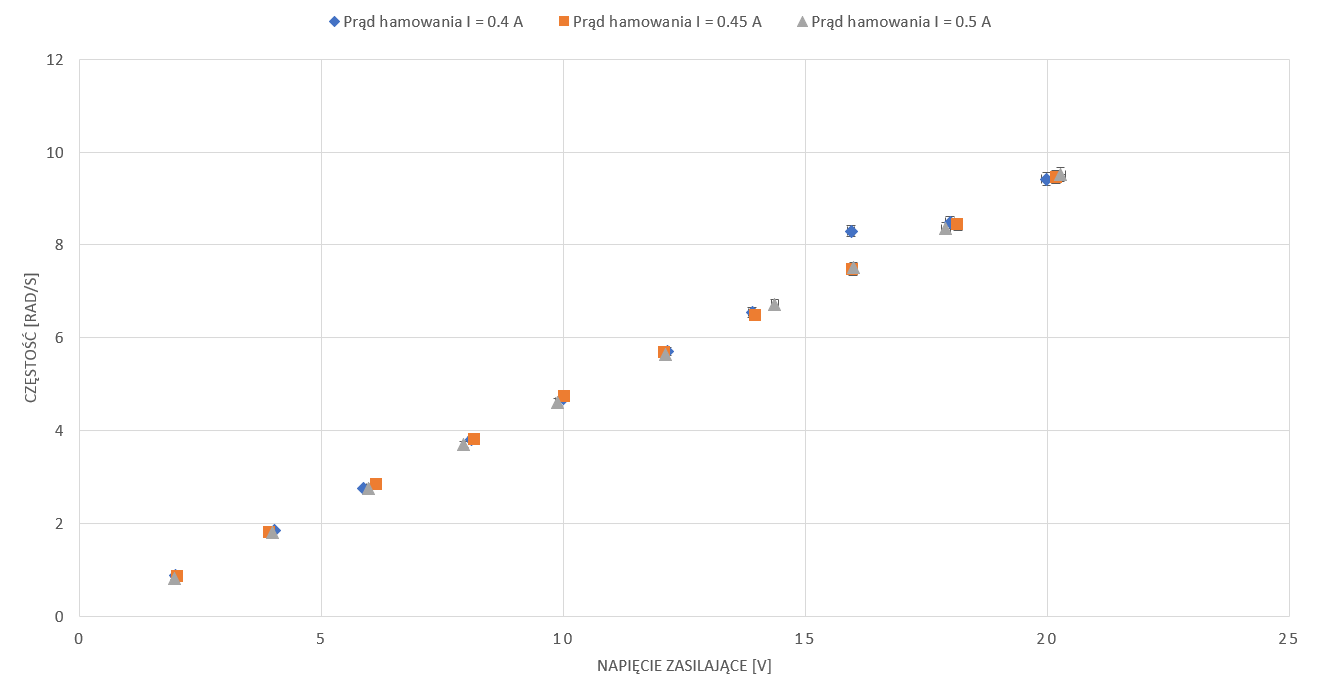
\includegraphics[scale=0.34]{f7.png}
\end{figure}

% Table generated by Excel2LaTeX from sheet 'Arkusz1'
\begin{table}[h]
  \centering
  \caption{Napięcie zasilające i amplituda drgań przy prądzie hamującym I = (0.320 $\pm$ 0.057) A}
    \begin{tabular}{|c|c|c|c|}\hline
    $U~[V]$ & $u(U)~[V]$ & $A~[dz]$ & $u(A)~[dz]$ \\\hline
    2.1630 & 0.0075 & 0.400 & 0.058 \\\hline
    3.371 & 0.012 & 0.400 & 0.058 \\\hline
    4.020 & 0.014 & 0.600 & 0.058 \\\hline
    5.200 & 0.017 & 0.900 & 0.058 \\\hline
    5.980 & 0.019 & 1.400 & 0.058 \\\hline
    6.620 & 0.021 & 4.200 & 0.058 \\\hline
    6.780 & 0.022 & 6.400 & 0.058 \\\hline
    6.890 & 0.022 & 9.200 & 0.058 \\\hline
    7.000 & 0.022 & 9.700 & 0.058 \\\hline
    7.140 & 0.023 & 5.500 & 0.058 \\\hline
    7.610 & 0.024 & 2.000 & 0.058 \\\hline
    8.550 & 0.027 & 0.800 & 0.058 \\\hline
    9.030 & 0.029 & 0.500 & 0.058 \\\hline
    10.310 & 0.032 & 0.200 & 0.058 \\\hline
    11.920 & 0.037 & 0.100 & 0.058 \\\hline
    12.690 & 0.040 & 0.050 & 0.058 \\\hline
    \end{tabular}%
  \label{tab:addlabel}%
\end{table}%
% Table generated by Excel2LaTeX from sheet 'Arkusz1'
\begin{table}[h]
  \centering
  \caption{Napięcie zasilające i amplituda drgań przy prądzie hamującym I = (0.270 $\pm$ 0.056) A}
    \begin{tabular}{|c|c|c|c|}\hline
    $U~[V]$ & $u(U)~[V]$ & $A~[dz]$ & $u(A)~[dz]$ \\\hline
    2.5690 & 0.0088 & 0.200 & 0.058 \\\hline
    3.161 & 0.011 & 0.200 & 0.058 \\\hline
    4.030 & 0.014 & 0.600 & 0.058 \\\hline
    5.190 & 0.017 & 0.800 & 0.058 \\\hline
    6.330 & 0.020 & 2.000 & 0.058 \\\hline
    6.440 & 0.021 & 3.100 & 0.058 \\\hline
    6.590 & 0.021 & 4.800 & 0.058 \\\hline
    6.780 & 0.022 & 8.800 & 0.058 \\\hline
    6.900 & 0.022 & 12.000 & 0.058 \\\hline
    6.950 & 0.022 & 12.800 & 0.058 \\\hline
    7.040 & 0.023 & 13.000 & 0.058 \\\hline
    7.210 & 0.023 & 6.400 & 0.058 \\\hline
    7.350 & 0.024 & 3.800 & 0.058 \\\hline
    7.540 & 0.024 & 2.600 & 0.058 \\\hline
    8.330 & 0.026 & 1.000 & 0.058 \\\hline
    9.290 & 0.029 & 0.600 & 0.058 \\\hline
    10.080 & 0.032 & 0.200 & 0.058 \\\hline
    10.850 & 0.034 & 0.100 & 0.058 \\\hline
    \end{tabular}%
  \label{tab:addlabel}%
\end{table}%

% Table generated by Excel2LaTeX from sheet 'Arkusz1'
\begin{table}[h]
  \centering
  \caption{Napięcie zasilające i amplituda drgań przy prądzie hamującym I = (0.210 $\pm$ 0.055) A}
    \begin{tabular}{|c|c|c|c|}\hline
    $U~[V]$ & $u(U)~[V]$ & $A~[dz]$ & $u(A)~[dz]$ \\\hline
    2.6180 & 0.0089 & 0.300 & 0.058 \\\hline
    3.498 & 0.012 & 0.400 & 0.058 \\\hline
    4.130 & 0.014 & 0.600 & 0.058 \\\hline
    4.950 & 0.016 & 0.800 & 0.058 \\\hline
    5.730 & 0.019 & 1.000 & 0.058 \\\hline
    6.600 & 0.021 & 4.000 & 0.058 \\\hline
    6.750 & 0.022 & 8.400 & 0.058 \\\hline
    6.900 & 0.022 & 15.000 & 0.058 \\\hline
    6.950 & 0.022 & 17.000 & 0.058 \\\hline
    7.000 & 0.022 & 18.800 & 0.058 \\\hline
    7.050 & 0.023 & 19.200 & 0.058 \\\hline
    7.190 & 0.023 & 19.800 & 0.058 \\\hline
    7.370 & 0.024 & 20.000 & 0.058 \\\hline
    7.510 & 0.024 & 20.000 & 0.058 \\\hline
    7.650 & 0.024 & 5.000 & 0.058 \\\hline
    8.240 & 0.026 & 1.400 & 0.058 \\\hline
    8.860 & 0.028 & 1.000 & 0.058 \\\hline
    9.250 & 0.029 & 0.600 & 0.058 \\\hline
    10.380 & 0.033 & 0.200 & 0.058 \\\hline
    11.160 & 0.035 & 0.100 & 0.058 \\\hline
    \end{tabular}%
  \label{tab:addlabel}%
\end{table}%

\begin{figure}[h]
\centering
\caption{Wykresy funkcji A = f(U) zestawione razem dla trzech wartości prądu hamowania}
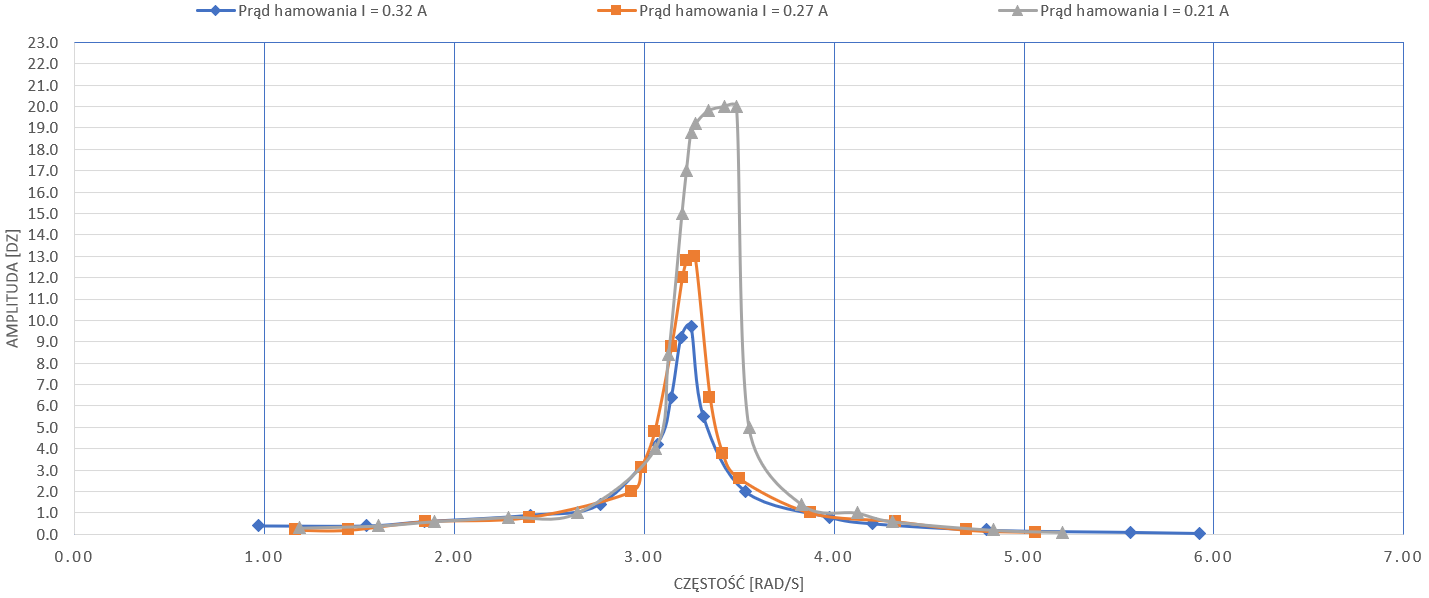
\includegraphics[scale=0.4]{f8.png}
\end{figure}
% Table generated by Excel2LaTeX from sheet 'Arkusz1'
\begin{table}[h]
  \centering
  \caption{Prąd hamujący, częstość rezonansowa, szerokość krzywej w połowie wysokości, dobroć układu}
    \begin{tabular}{|c|c|c|c|c|c|c|c|}\hline
    $I~[A]$&$u(I)~[A]$&$\omega_r~[rad/s]$ & $u(\omega_r)~[rad/s]$ & $\Delta\omega$ & $u(\Delta\omega)$ & $Q$ & $u_C(Q)$ \\\hline
    0.210&0.055&3.3 & 0.1 & 0.460 & 0.025 & 7.17 & 0.45 \\\hline
    0.270&0.056&3.3 & 0.1 & 0.520 & 0.025 & 6.35 & 0.37 \\\hline
    0.320&0.057&3.5 & 0.1 & 0.780 & 0.025 & 4.5 & 0.2 \\\hline
    \end{tabular}%
  \label{tab:addlabel}%
\end{table}%


\clearpage
\section{Wnioski}
\begin{itemize}
\item Wyznaczone częstości własne dla różnych wychyleń początkowych są zbieżne, można więc wnioskować brak zależności częstości własnej od wartości wychylenia początkowego.
\item Na podstawie samych wykresów można zauważyć wpływ prądu hamującego na czas ustania oscylacji - im większy prąd, tym szybciej drgania wygasają, co potwierdzają dalsze obliczenia.
\item Wartość logarytmicznego dekrementu tłumienia układu $\Lambda_{swobodny}$ = 0.158 $\pm$ 0.011
\item Wartość logarytmicznego dekrementu tłumienia układu $\Lambda_{I_1}$ = 0.34 $\pm$ 0.04, przy prądzie hamującym I$_1$ = (0.46 $\pm$ 0.06) A
\item Wartość logarytmicznego dekrementu tłumienia układu $\Lambda_{I_2}$ = 0.29 $\pm$ 0.15, przy prądzie hamującym I$_2$ = (0.400 $\pm$ 0.058) A
\item Na podstawie rysunków 4 - 6 stwierdzono, że silniczek ma liniową charakterystykę.
\item Na podstawie rysunku 7 stwierdzono, że częstość silniczka nie zależy od prądu hamowania, ponieważ dla trzech wartości prądów hamowania częstości przyjmują taką samą wartość dla tych samych wartości napięcia zasilającego.
\item Układ, niezależnie od prądu hamującego, wpada w rezonans dla napięcia U = 7 V, co odpowiada częstości rezonansowej około $\omega_{rez}$ = 3.3 $\frac{rad}{s}$ (odczyt z rys. 5).
\item Wyniki pomiarów zaprezentowane na rys. 8 przybliżone zostały krzywymi dla lepszego zobrazowania oczekiwanych krzywych dzwonowych.
\item Częstość rezonansowa oraz szerokość dzwonu odczytane zostały po zagęszczeniu siatki i znacznym przybliżeniu rysunków 5 oraz 8.
\item Dobroć układu przy prądzie hamującym I = (0.320 $\pm$ 0.057) A, wynosi Q = 4.5 $\pm$ 0.2.
\item Dobroć układu przy prądzie hamującym I = (0.270 $\pm$ 0.056) A, wynosi Q = 6.35 $\pm$ 0.37.
\item Dobroć układu przy prądzie hamującym I = (0.210 $\pm$ 0.055) A, wynosi Q = 7.17 $\pm$ 0.45.
\end{itemize}
\end{document}